\paragraph{Sơ đồ tuần tự luồng kích hoạt xác thực 2 lớp}

Luồng nghiệp vụ này mô tả
chi tiết quá trình người dùng
thiết lập mã xác thực hai lớp (2FA)
sử dụng giao thức TOTP (Time-based One-Time Password)
qua Supabase Service.

\subparagraph{Mô tả tổng quan}

\begin{itemize}

\item \textbf{Yêu cầu thiết lập 2 lớp:}
Người dùng
chọn kích hoạt xác thực hai lớp.
Giao diện gửi yêu cầu đăng ký qua cổng API đến Auth Service.
Auth Service đăng ký thiết bị xác thực mới
ở trạng thái chưa kiểm chứng,
đồng thời tạo mã khóa bảo mật và hình ảnh mã QR gửi về giao diện.

\item \textbf{Đồng bộ hóa ứng dụng:}
Người dùng
quét hình ảnh QR
bằng ứng dụng xác thực trên điện thoại
để thiết lập đồng bộ thời gian.
Ứng dụng này sẽ liên tục tạo ra các mã xác thực gồm sáu chữ số thay đổi mỗi ba mươi giây.

\item \textbf{Nhập mã kiểm chứng:}
Người dùng
nhập mã xác thực hiển thị trên ứng dụng để kiểm tra.
Giao diện gửi yêu cầu tạo mã thách thức
và gửi mã xác thực kèm mã thách thức qua cổng API tới Auth Service để xác minh.

\item \textbf{Kích hoạt thành công:}
Nếu mã xác thực chính xác,
Auth Service chuyển trạng thái
thiết bị xác thực thành đã xác minh,
đồng thời cấp lại mã đăng nhập mới
với mức độ bảo mật cao hơn cho người dùng.
\end{itemize}

\begin{figure}[H]
\centering
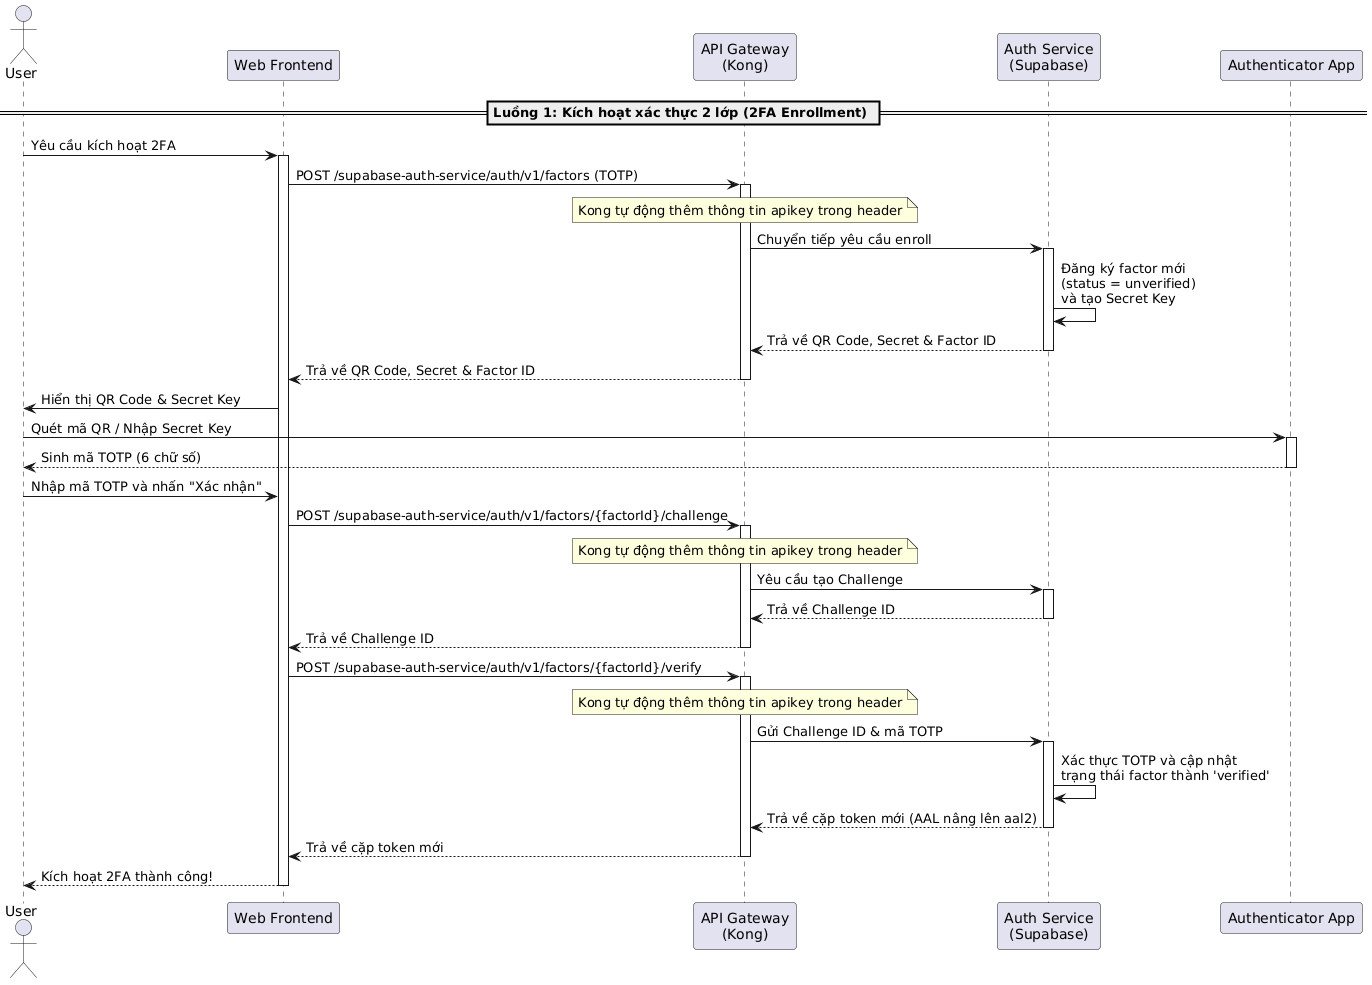
\includegraphics[width=0.95\textwidth]{contents/Sequence/UML-Sequence-UserMfaEnrollment.png}
\caption{Sơ đồ tuần tự luồng kích hoạt xác thực 2 lớp}
\end{figure}

\begin{table}[H]
\centering
\renewcommand{\arraystretch}{1.3}

\begin{tabular}{|l|l|p{5cm}|}
\hline
\textbf{Thành phần} & \textbf{Phân loại} & \textbf{Vai trò trong hệ thống} \\ \hline
User & Actor & Người dùng thực hiện kích hoạt xác thực 2 lớp. \\ \hline
Web Frontend & Component & Giao diện web Next.js. \\ \hline
API Gateway (Kong) & Component & Cổng API chuyển tiếp các yêu cầu API. \\ \hline
Auth Service (Supabase) & Microservice & Dịch vụ xác thực sinh mã bí mật và xác minh TOTP. \\ \hline
Authenticator App & External Service & Ứng dụng di động (Google Authenticator...) quét QR sinh mã TOTP. \\ \hline
\end{tabular}
\caption{Các thành phần tham gia luồng kích hoạt xác thực 2 lớp}
\end{table}
